\chapter{Clusterização} \label{cap:clusterizacao}

A clusterização é denominada como técnica para organização ou agrupamento de uma coleção de padrões, ou elementos que sigam padrões, em \textit{clusters} baseada em similaridade.
Trata-se de uma técnica bastante utilizada em análise exploratórias, agrupamentos, tomada de decisão e implementações de \textit{machine learning}, como:
mineração de dados, recuperação de documentos, segmentação de imagens e padronização \cite{clustering_review}.

A aplicação da técnica pode ser resumida nos passos apresentados na Figura \ref{fig:tasks_clustering}.

\begin{figure}[h!]
\centering
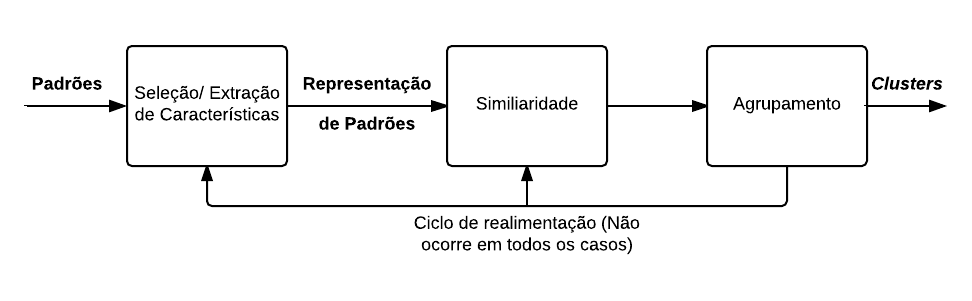
\includegraphics[scale=0.6]{figuras/tasks_clustering.png}
\caption{Passos para clusterização. Adaptado de \citeonline{clustering_review}}
\label{fig:tasks_clustering}
\end{figure}

A representação de padrões está relacionada ao número de classes, número de padrões disponíveis e o número, tipo e escala
das características disponíveis no algoritmo de clusterização. Algumas dessas informações podem não ser controladas pelos
profissionais \cite{clustering_review}.

A seleção de características é o processo de identificação do subconjunto das características mais eficaz para a clusterização, já a extração
de características é o uso de uma ou mais transformações das características de entrada para produzir novas características \cite{clustering_review}.

A similaridade, em geral, é medida por uma função de distância entre um par de padrões ou elementos. Essa função de distância pode variar
de acordo com o contexto da aplicação. E por fim, o agrupamento pode ser realizado com uso de vários algoritmos diferentes \cite{clustering_review}.

